\lab{Intro to IVP and BVP}{Intro to IVP and BVP}
\label{lab:BVPIntro}
\labdependencies{}

\section*{Initial Value Problems}

An initial value problem is a differential equation with a set of constraints at the initial point.
An IVP may look something like this
\begin{align*}
    y'' + y' + y &= f(t) \\
    y(a) &= \alpha \\
    y'(a) &= \beta \\
    t \in &[a,b].
\end{align*}
This problem gives a differential equation with initial conditions for $y$ and $y'$.

Formulating and solving initial value problems is an important tool when solving many types of problems.
One simple example of an IVP would be a differential equation modeling the path of a ball thrown in the air where the initial position ($y(a)$) and velocity ($y'(a)$) are known.
These problems can be tricky to solve by hand.
Luckily, SciPy has great tools that help us solve initial value problems for most systems of first order ODEs.
We will be using \li{solve_ivp} from \li{scipy.integrate}.

Consider the following example
\begin{equation*}
    y''+3y = \sin(t), \quad
    y(0) = -\pi /2, \quad
    y'(0) = \pi, \quad
    t \in [0,5]
\end{equation*}
We begin by changing this second order ODE into a first order ODE system.
\begin{align*}
    \text{Let } y_1 = y &\text{ and } y_2 = y' \text{ so that}\\
    \begin{bmatrix}
        y_1\\y_2
    \end{bmatrix}'
    &=
    \begin{bmatrix}
        y_2 \\
        \sin{t} - 3y_1
    \end{bmatrix}.
\end{align*}
This formulation allows us to use \li{solve_ivp}.
We need three code elements in order to use \li{solve_ivp}:
\begin{enumerate}
    \item The ODE function: \\
    This function defines the right-hand side of the ODE system, and returns an array containing its values for our first order system of ODEs.
    \item The time domain: \\
    This is a tuple giving the interval of integration. 
    \item The initial conditions: \\
    This is an array containing the initial conditions of each coordinate of the ODE.
    In our example, these are the value of the "zeroeth" derivative, followed by the first derivative, and so on if there are higher order derivatives. 
\end{enumerate}
The following code sets up and solves the IVP in the above example:
\begin{lstlisting}
from scipy.integrate import solve_ivp
import numpy as np

# element 1: the ODE function
def ode(t, y):
    '''defines the ode system'''
    return np.array([y[1],np.sin(t)-3*y[0]])
    
# element 2: the time domain
t_span = (0,5)

# element 3: the initial conditions
y0 = np.array([-np.pi /2, np.pi])

# solve the system
# max_step is an optional parameter that controls maximum step size and 
# a smaller value will result in a smoother graph
sol = solve_ivp(ode, t_span, y0, max_step=0.1)

# as an alternative, the parameter t_eval can be used to evaluate the function
# at specific points; this can also be used to get a smooth graph
sol = solve_ivp(ode, t_span, y0, t_eval=np.linspace(0, 5, 150))
\end{lstlisting}
Then we can plot the solution with the following code:
\begin{lstlisting}
from matplotlib import pyplot as plt

plt.plot(sol.t,sol.y[0])
plt.xlabel('t')
plt.ylabel('y(t)')
plt.show()
\end{lstlisting}

\begin{figure}[H]
    \centering
%    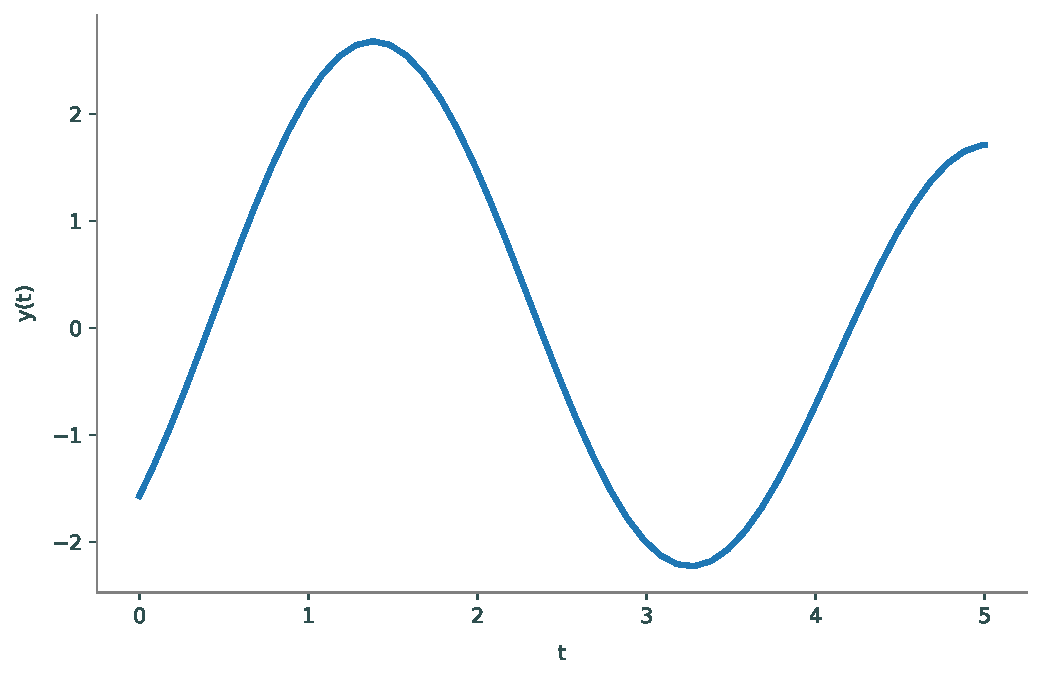
\includegraphics[width=\textwidth]{figures/fig1.pdf}
    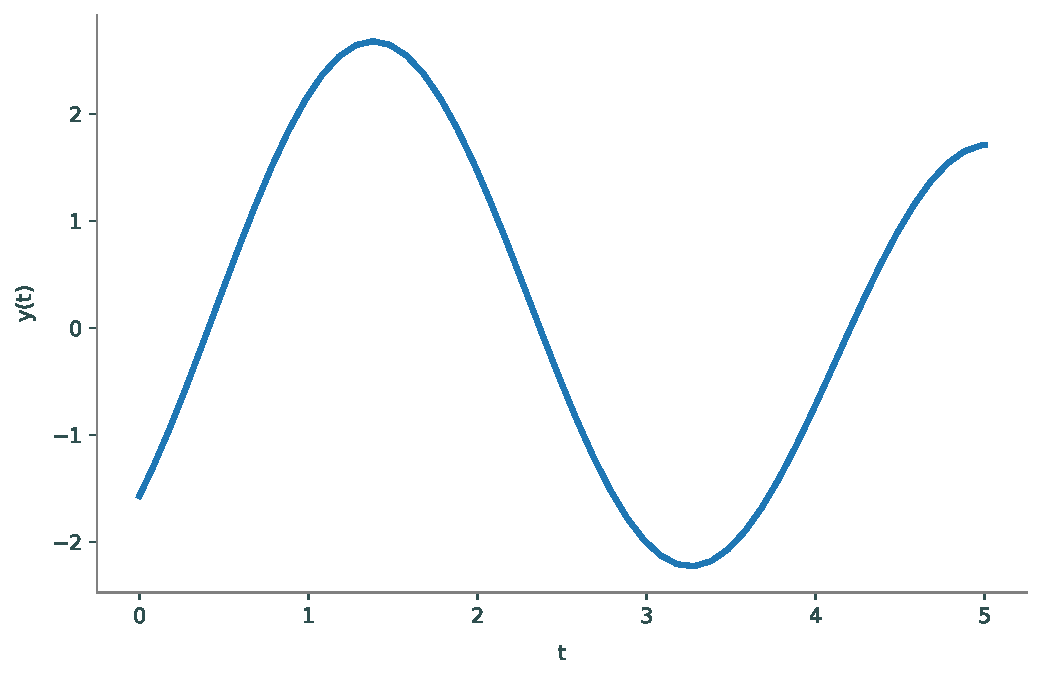
\includegraphics[height=3in]{figures/fig1.pdf}
    \caption{The solution to the above example}
\end{figure}

\begin{problem}
\label{prob:bvpintro:bvp1}
Use \li{solve_ivp} to solve for $y$ in the equation $y'' - y = \sin(t)$ with initial conditions $y(0)= -\frac{1}{2}$, $y'(0) = 0$ and plot your solution on the interval $[0,5]$.
Compare this to the analytic solution $y=-\frac{1}{2}(e^{-t}+\sin(t))$.

    Note: Using \li{max_step} = 0.1 with give you the smoother graph seen in figure \ref{fig:bvpintro:bvp1}.
\end{problem}

\begin{figure}[H]
    \centering
   % 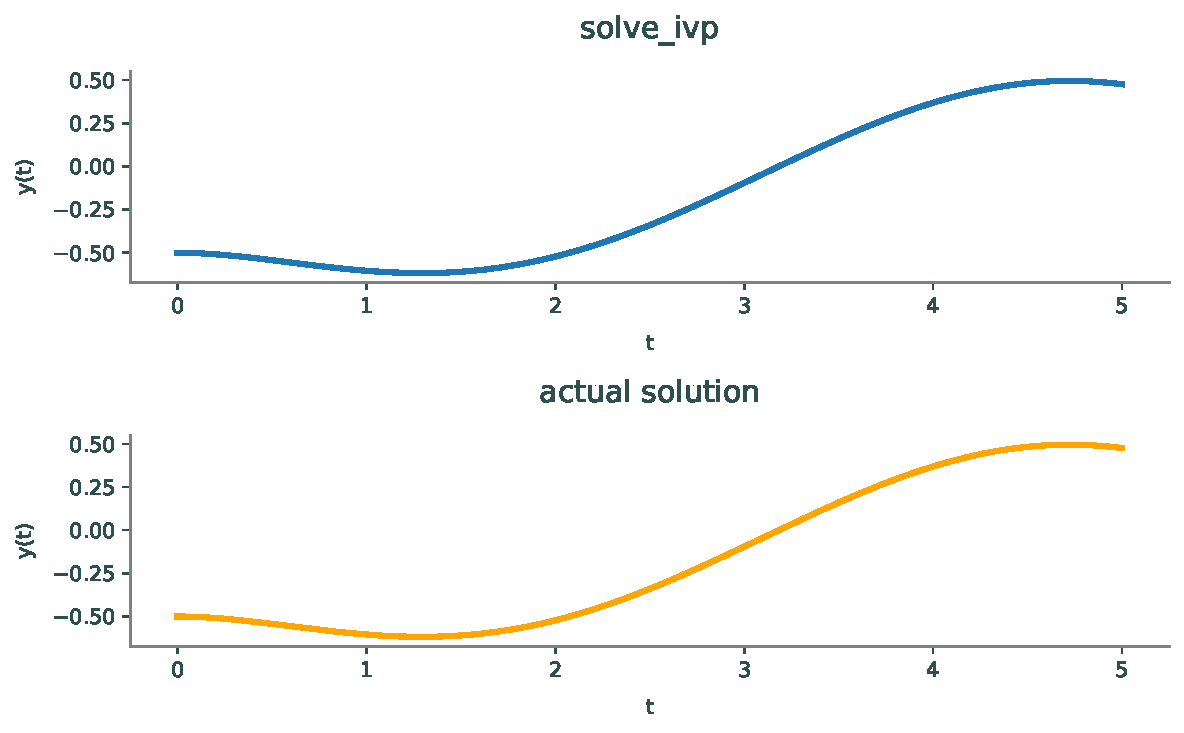
\includegraphics[width=\textwidth]{figures/problem1.pdf}
    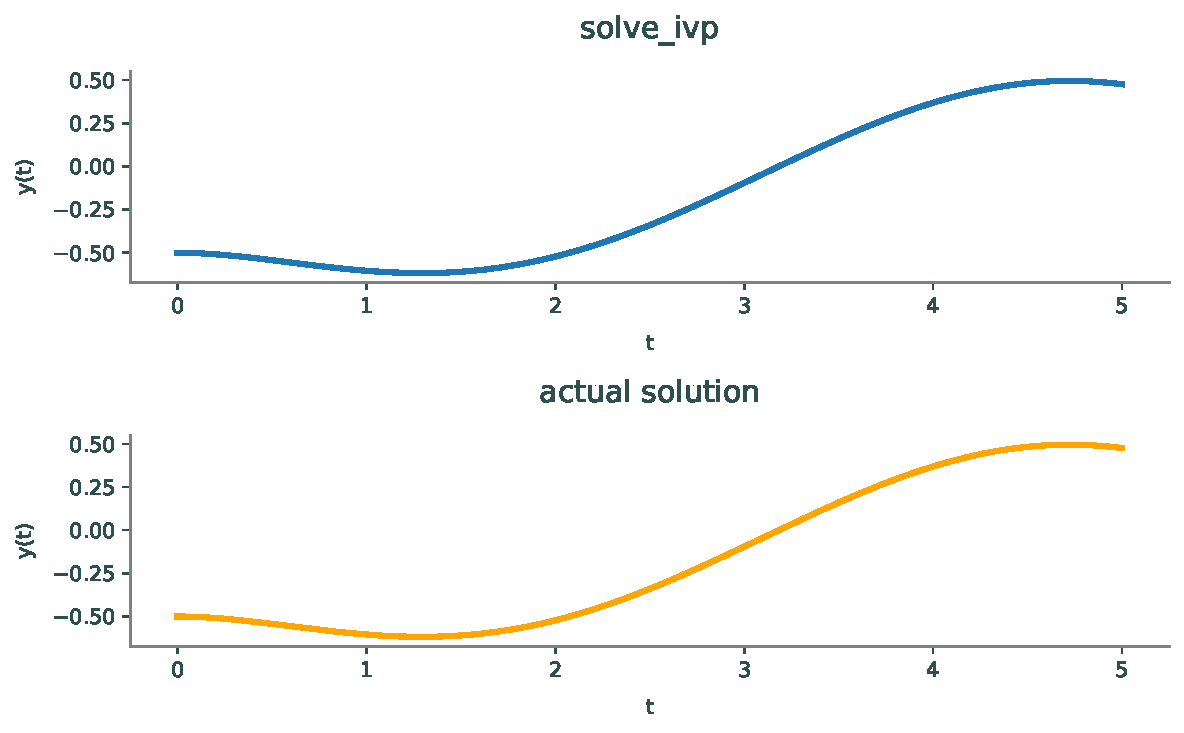
\includegraphics[height=3in]{figures/problem1.pdf}
    \caption{The solution to Problem \ref{prob:bvpintro:bvp1}}
    \label{fig:bvpintro:bvp1}
\end{figure}

\section*{Boundary Value Problems}
A boundary value problem is a differential equation with a set of constraints.
It is similar to initial value problems, but may give end constraints as well as initial constraints.
A boundary value problem may look something like this
\begin{align*}
    y'' + y' + y &= f(t) \\
    y(a) &= \alpha \\
    y(b) &= \beta \\
    t\in &[a,b],
\end{align*}
where we have both right and left hand boundary conditions on $y$.
One simple example of a BVP would be a differential equation modeling the path of a ball thrown in the air where the initial position ($y(a)$) and final position ($y(b)$) are known. Note that like an IVP problem, a BVP problem has two boundary conditions.

SciPy has great tools that help us solve boundary value problems.
We will be using \li{solve_bvp} from \li{scipy.integrate}.
Consider the following example:
\begin{equation}
    y'' + 9y = \cos(t),\quad
    y'(0) = 5, \quad
    y\left(\pi\right) = -\frac{5}{3}.
\end{equation}
We begin by changing this second order ODE into a first order ODE system.
\begin{align*}
    \text{Let } y_1 = y &\text{ and } y_2 = y' \text{ so that,}\\
    \begin{bmatrix}
        y_1\\y_2
    \end{bmatrix}'
    &=
    \begin{bmatrix}
        y_2 \\
        \cos{t} - 9y_1
    \end{bmatrix}.
\end{align*}
This formulation allows us to use \li{solve_bvp}.
It is important to notice that there are several key differences between \li{solve_ivp} and \li{solve_bvp}.
We need four code elements in order to use \li{solve_bvp}:
\begin{enumerate}
    \item The ODE function: \\
    This is essentially the same function we used in \li{solve_ivp}.\footnote{There is a technical difference between how the two methods call the ODE function. Unlike \lif{solve_ivp}, \li{solve_bvp} calls the function on \emph{all} of the time steps all at once, so \lif{t} will be an array and \lif{y} will be a \((n,T)\) array where \(n\) is the dimension of the ODE and \(T\) is the number of timesteps. For most applications, this leads to no difference in how you code the ODE function, as can be seen in the examples; however, for some applications, such as piecewise ODE functions, this fact must be taken into consideration.}
    \item The boundary condition function: \\
    Instead of just having a tuple containing our initial values, we now must use a function that returns an array of the residuals of the boundary conditions. 
    We pass in 2 arrays: \li{ya}, representing the initial values, and \li{yb}, representing the final values. The \(i\)th entry of those arrays represents the boundary condition at the \(i\)th coordinate of the ODE.
    Returning \li{ya[0]-x} would indicate that we know \(y_1(a)=x\), \li{ya[1]-x} would indicate that we know \(y_2(a)=x\), \li{yb[0]-x} would indicate that we know \(y_1(b)=x\), and \li{yb[1]-x} would indicate that we know \(y_2(b)=x\).
    \item The time domain: \\
    Instead of a tuple giving the interval of integration, we now must pass in a linspace from the starting time to the ending time, containing the desired number of points (we now must choose the number).
    As part of its algorithm, \li{solve_bvp} will add additional points to the mesh to attempt to reduce the error of the approximation, so it is not generally necessary to pass in a very fine mesh.
    This also means that the mesh of the returned solution will generally not be the same as the one you pass in here.
    \item The initial guess: \\
    As we no longer know all of the initial values, we now must make a (hopefully educated) guess. This is an array of shape \li{(n, t_steps)} where \li{n} is the shape of the output of the ODE function and \li{t_steps} is the chosen number of steps in our time domain linspace. 
\end{enumerate}

\begin{lstlisting}
from scipy.integrate import solve_bvp
import numpy as np

# element 1: the ODE function
def ode(t,y):
    ''' define the ode system '''
    return np.array([y[1], np.cos(t) - 9*y[0]])
# element 2: the boundary condition function
def bc(ya,yb):
    ''' define the boundary conditions '''
    # ya are the initial values
    # yb are the final values
    # each entry of the return array will be set to zero
    return np.array([ya[1] - 5, yb[0] + 5/3])

# element 3: the time domain.
t_steps = 100
t = np.linspace(0,np.pi,t_steps)

# element 4: the initial guess.
y0 = np.ones((2,t_steps))

# Solve the system.
sol = solve_bvp(ode, bc, t, y0)
\end{lstlisting}
%
The syntax for plotting the function is also slightly different:
\begin{lstlisting}
import matplotlib.pyplot as plt

# here we plot sol.x instead of sol.t
plt.plot(sol.x, sol.y[0])
plt.xlabel('t')
plt.ylabel('y(t)')
plt.show()
\end{lstlisting}

\begin{figure}[H]
    \centering
    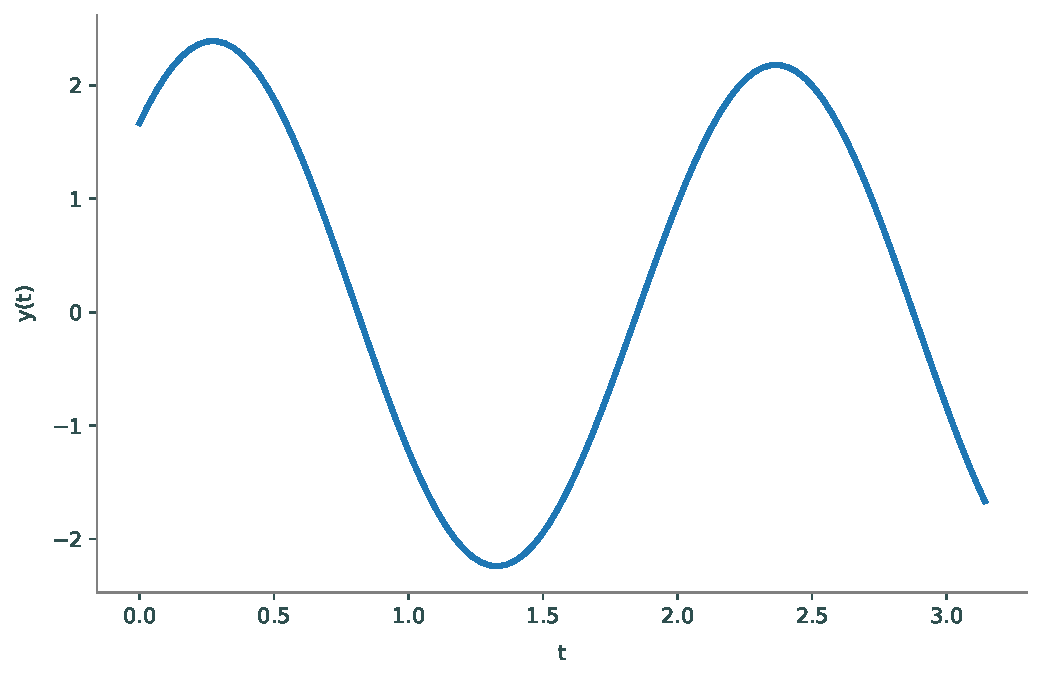
\includegraphics[height=3in]{figures/fig3.pdf}
    \caption{The solution to the above boundary value problem}
\end{figure}

\begin{problem}
    \label{prob:bvpintro:bvp2}
    Use \li{solve_bvp} to solve for $y$ in the equation $y'' + y' = -\frac{1}{4}e^{-t/2}+\sin(t)-\cos(t)$ with boundary conditions $y(0)= 6$, $y'(5) = -0.324705$ and plot your solution on the interval $[0,5]$. Compare this to the analytic solution $y=e^{-t/2}-\sin(t)+5$.
\end{problem}

\begin{figure}[H]
\label{fig:bvpintro:bvp2}
    \centering
    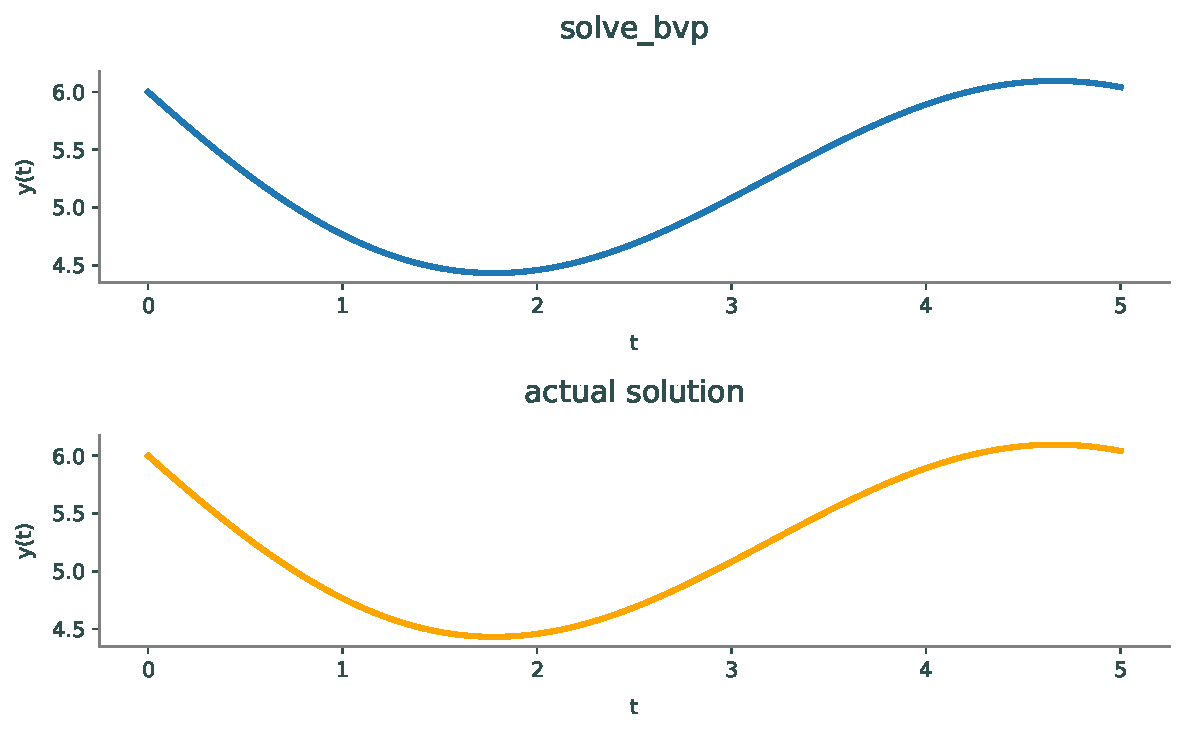
\includegraphics[height=3in]{figures/problem2.pdf}
    \caption{The solution to problem \ref{prob:bvpintro:bvp2}.}
\end{figure}

One other useful functionality of \li{solve_bvp}: \li{sol.sol} is a callable function, which is the estimation of the boundary value problem. 
You can plug in any value or numpy array (\li{sol.sol(np.linspace)}, \li{sol.sol(float)}, \li{sol.sol(list)}), like a normal lambda function.

\section*{The Pitfalls of \li{solve_bvp}}
One of the common issues with \li{solve_bvp} is choosing a guess for the initial value.
Often, small changes in the guess can cause large changes in the final approximation. 
The reason for this is that the algorithm used by \li{solve_bvp} is essentially a version of Newton's method set up to approximate the boundary value problem, and thus can be sensitive to the initial guess.
The next problem demonstrates the huge difference that can be made between a constant initial guess of $10$ and a constant initial guess of $9.99$

\begin{problem}
    \label{prob:bvpintro:bvp3}
    Use \li{solve_bvp} to solve for $y$ in the equation $y''=(1-y')*10y$ with boundary conditions $y(0)=-1$ and $y(1)=\frac{3}{2}$ and plot your solution on the interval $[0,1]$. Use an initial guess of 10.
    Compare this to the the same solution using an initial guess of 9.99.
    For both of your initial guesses, use 50 steps in \(t\).

    The solution is found in Figure \ref{fig:bvpintro:bvp3}.
\end{problem}

\begin{figure}[H]
    \centering
    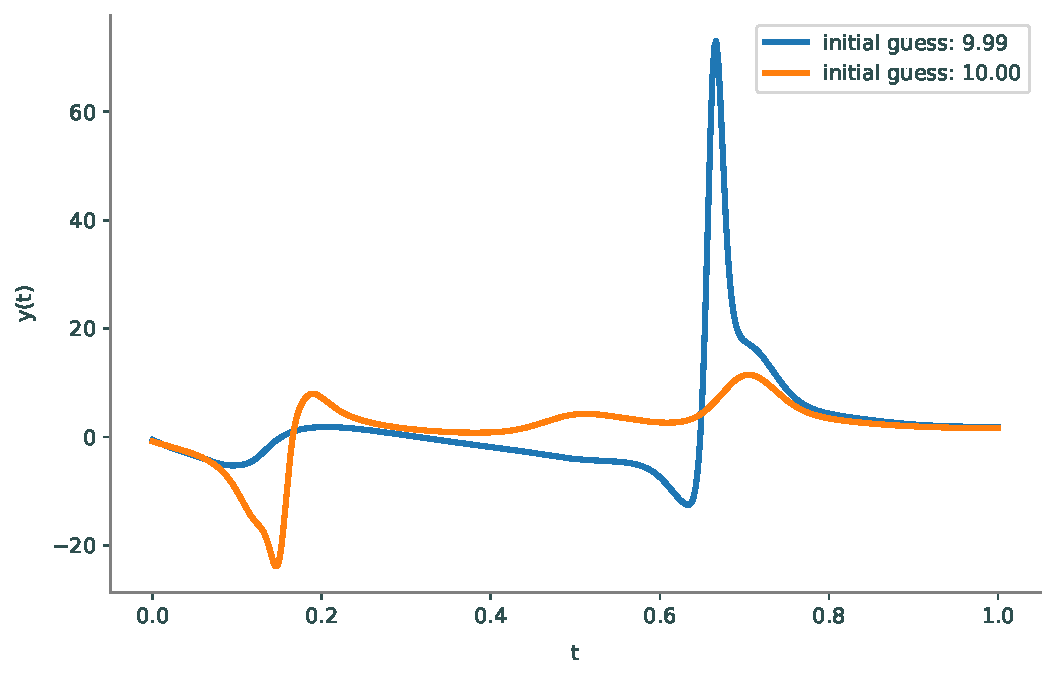
\includegraphics[height=3in]{figures/problem3.pdf}
    \caption{The solution to problem \ref{prob:bvpintro:bvp3}.}
    \label{fig:bvpintro:bvp3}
\end{figure}

\section*{Strange Attractors}
In the growing field of dynamical systems, an attractor is a set of states toward which a system tends to evolve.
Strange attractors are special in that they showcase complex behavior in a simple set of equations.
A minute change in the initial values can cause massive differences in the outcome.
The most famous of these is the Lorenz attractor, introduced by Edward Lorenz in 1963.
Later on, we dedicate a full lab to the study of the Lorenz attractor, but today we focus on modeling the Four-Wing attractor.
This is a system of first order ODEs defined by the following set of equations
\begin{align}
    \frac{dx}{dt} &= ax + yz \label{eq:IVP_BVP_Intro:lorenz_dxdt} \\
    \frac{dy}{dt} &= bx + cy - xz \label{eq:IVP_BVP_Intro:lorenz_dydt} \\
    \frac{dz}{dt} &= -z - xy \label{eq:IVP_BVP_Intro:lorenz_dzdt} 
\end{align}
given some constants $a$, $b$, and $c$.
As we mentioned earlier, \li{solve_ivp} and \li{solve_bvp} can be used to solve and model systems of first order ODEs. We will now use \li{solve_ivp} to model the Four-Wing attractor.

\begin{problem}
    \label{prob:bvpintro:bvp4}
Use \li{solve_ivp} to solve the Four-Wing Attractor as described in equations \eqref{eq:IVP_BVP_Intro:lorenz_dxdt}, \eqref{eq:IVP_BVP_Intro:lorenz_dydt}, and \eqref{eq:IVP_BVP_Intro:lorenz_dzdt} where $a=0.2$, $b = 0.01$, and $c = -0.4$. Try this with 3 different initial values and plot (in three dimensions) the 3 corresponding graphs.

Examples of solutions are given in Figure \ref{fig:bvpintro:bvp4}.

Hint: Because the attractor lies mostly within the box $[-2,2]^2$, it is best to have the initial conditions also within this box. Also, you may need the time scale to run from about about $0$ to $400$ to visualize the full attractor.
\end{problem}

\begin{figure}[H]
    \begin{subfigure}[b]{.3\textwidth}
        \centering
        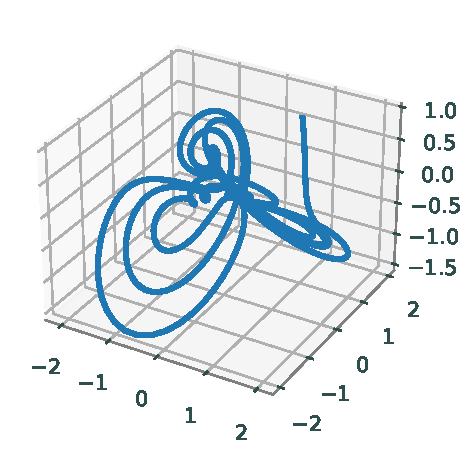
\includegraphics[width = \textwidth]{figures/problem41.pdf}
    \end{subfigure}
    \begin{subfigure}[b]{.3\textwidth}
        \centering
        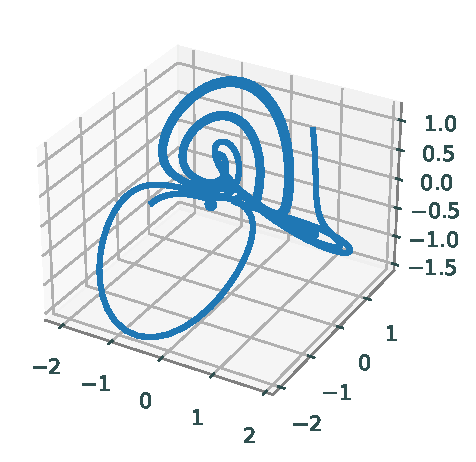
\includegraphics[width = \textwidth ]{figures/problem42.pdf}
    \end{subfigure}
    \begin{subfigure}[b]{.3\textwidth}
        \centering
        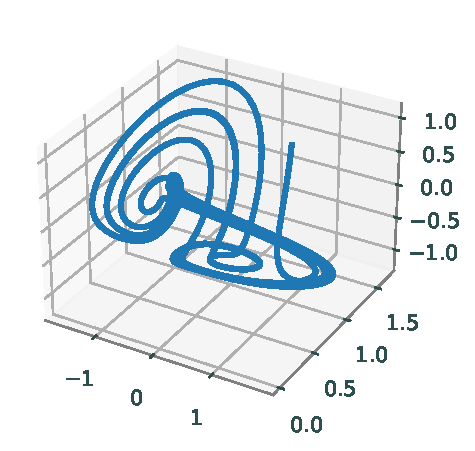
\includegraphics[width = \textwidth ]{figures/problem43.pdf}
    \end{subfigure}
    \caption{Possible solutions to problem 4.}
    \label{fig:bvpintro:bvp4}
\end{figure}


\section*{BVPs with Free Parameters}

The function \li{solve_bvp} also supports solving for free parameters in a boundary value problem.
The syntax is very similar to what we did above, except that our functions will have an additional argument that is a list of all of the free parameters.
For example, suppose we have the following BVP with free parameter \(a\), that is, in addition to the BVP, we are also solving for an unknown parameter \(a\):
\begin{align*}
x'(t) &= (1+t)y(t)-x(t) \\
y'(x) &= a\sin(x(t))
\\
x(0)=1&,\; x(1)=0,\; y(1)=2
\end{align*}
Note that we need one additional boundary condition for each free parameter; in this case, since we have two variables and one free parameter, we need three boundary conditions.
We set up the ODE and boundary condition functions as follows:
\begin{lstlisting}
# The ODE function
def ode(t, y, p):
    ''' Defines the ODE system '''
    return np.array([
        (1+t)* y[1] - y[0],
        p[0] * np.sin(y[0])
    ])

# The boundary condition function
def bcs(ya, yb, p):
    ''' Defines the boundary conditions '''
    return np.array([
        ya[0] - 1,
        yb[0] - 0,
        yb[1] - 2
    ])
\end{lstlisting}
Note that both of these functions accept an additional argument \li{p}, which is a list of the free parameters in the problem.
In this case, we only have one parameter, so \li{p=[a]}.
Using \li{solve_bvp} to get the solution is similar to before, except that we must also pass in a guess for the free parameters with the argument \li{p}:
\begin{lstlisting}
# Guess of the solution values
t = np.linspace(0, 1, 50)
y_guess = np.ones((2,50))
p_guess = [1]

# Solve
sol = solve_bvp(ode, bcs, t, y_guess, p=p_guess)
\end{lstlisting}
The solution can be plotted as before, and the value of the free parameters for the solution can be found with \li{sol.p}:
\begin{lstlisting}
plt.plot(sol.x, sol.y[0], label='$x(t)$')
plt.plot(sol.x, sol.y[1], label='$y(t)$')
plt.legend()
plt.xlabel('t')
plt.ylabel('y(t)')
plt.title(f'$a = {sol.p[0]:.4f}$')
plt.show()
\end{lstlisting}

\begin{figure}[H]
    \centering
    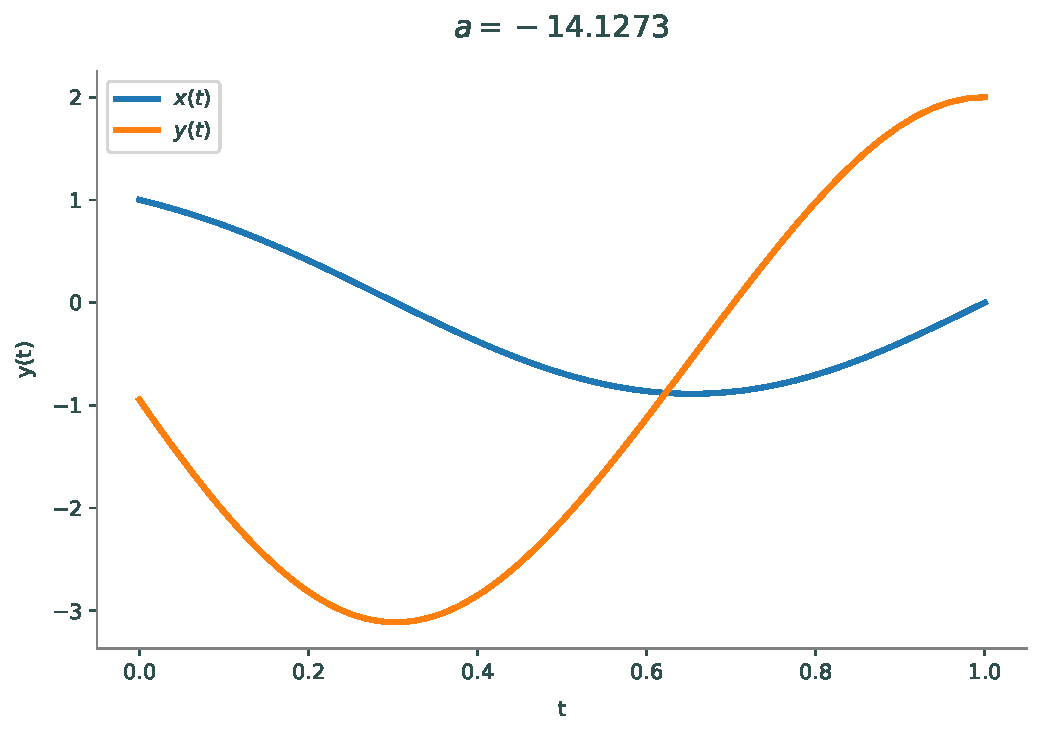
\includegraphics[height=3in]{figures/bvp_param_example.pdf}
    \caption{The solution to the above example}
\end{figure}

Free parameters occur in eigenvalue problems for differential operators.
The general form of these is
\begin{align*}
Dy&=\lambda y \\
y(a)=&y(b)=0
\end{align*}
where \(D\) is some differential operator and \(\lambda\) is an unknown scalar.
These differential eigenvalue problems are very analogous to the finite-dimensional case of matrix eigenvalue problems, except that instead of trying to find eigenvectors, we now try to find \textit{eigenfunctions}.
As in the matrix case, we are not interested in the trivial solution \(y=0\).
Furthermore, if we have an eigenfunction \(y\), any multiple \(ay\) is also an eigenfunction.
To solve both of these issues, we will stipulate that \(y'(a)=1\); this guarantees the solution is not identically zero, and also makes it unique for a given value of \(\lambda\). % if \(p,q\), and \(r\) are sufficiently nice.

\textit{Sturm-Liouville problems} are an important category of these eigenvalue problems.
These have the special form
\begin{align*}
(py')'+qy = \lambda ry \\
y(a)=y(b)=0
\end{align*}
where \(p(t), q(t), r(t)\) are known functions and \(\lambda\) is an unknown scalar.
Sturm-Liouville problems and their extensions are important theoretically, and their solutions have some very nice properties.
They also have applications in PDEs and occur in areas such as physics and quantum mechanics.

\begin{problem}
\label{prob:IVP_BVP_Intro:schroedinger}
An important problem in quantum mechanics is to find steady-state solutions of the Schr\"odinger equation.
These functions are solutions to the \textit{time-independent Schr\"odinger equation}.
This equation is a differential equation for the wave function \(\psi\), with one free parameter \(E\).
In one dimension, this equation is
\begin{equation}
\label{eq:IVP_BVP_Intro:schroedinger}
-\frac{\hbar^2}{2m}\psi''(x)+U(x)\psi(x)=E\psi(x)
\end{equation}
where \(U\) is a known function describing the potential energy. 
Note that this is in fact a Sturm-Liouville problem.
If a function \(\psi\) and scalar \(E\) satisfy this equation, they describe an allowed steady state of a particle in the system.
The value of \(E\) is the energy of the particle in that state, and the values of \(\psi\) are related to the probability of the particle being in any given location.
For simplicity, we will let \(\frac{\hbar^2}{2m}=1\).\footnote{Making constants equal to one in this way is acutally done quite frequently in particle physics, by choosing the units we are using appropriately.}

%Rewrite the ODE as a first order system.
Write a function that uses \li{solve_bvp} to find \(\psi\) and \(E\) that are solutions to \eqref{eq:IVP_BVP_Intro:schroedinger} for the potential \(U(x)=x^2\) and with boundary conditions \(\psi(-1)=\psi(1)=0, \psi'(-1)=1\).
By varying your initial guess for \(E\), use your function to find solutions for several different values of \(E\), and plot them together.
\end{problem}

\begin{figure}[H]
    \label{fig:bvpintro:bvp5}
    \centering
    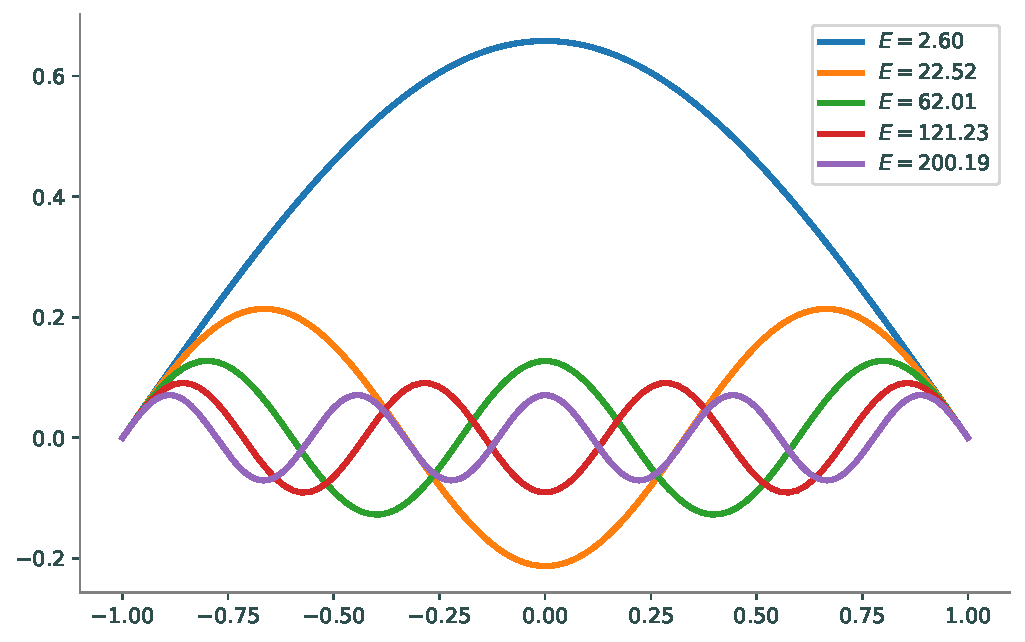
\includegraphics[height=3in]{figures/problem5.pdf}
    \caption{A possible solution to problem \ref{prob:IVP_BVP_Intro:schroedinger}.}
\end{figure}